\chapter{Detector Response to $^{14}$C Beta Decay}

The carbon-14 calibration follows the same preparation and injection procedure as the tritium calibration, which has been described in previous papers\cite{lux_tritium,richard,attila}. Both of these calibration sources have half-lives greater than the lifetime of the experiment, so we rely on the LUX gas processing system to chemically remove the injected activity. We have previously characterized our ability to remove radio-labelled methane from the LUX detector and found that tritiated-methane (CH$_3$T) is removed with a decay time of about 7-10 hours, leaving no observed residual activity in the detector. Carbon-14 labelled methane ($^{14}$CH$_4$) is chemically identical to CH$_3$T and so we find it to have the same removal characteristics. The tritiated methane is removed with a time constant of 8.2 hours, and the carbon-14 labeled methane is removed with a time constant 9.1 hours. This variation in removal time is within reason given the variation in previous trials with tritiated methane.
\begin{figure}[h!]
\centering
\begin{subfigure}{0.5\textwidth}
  \centering
  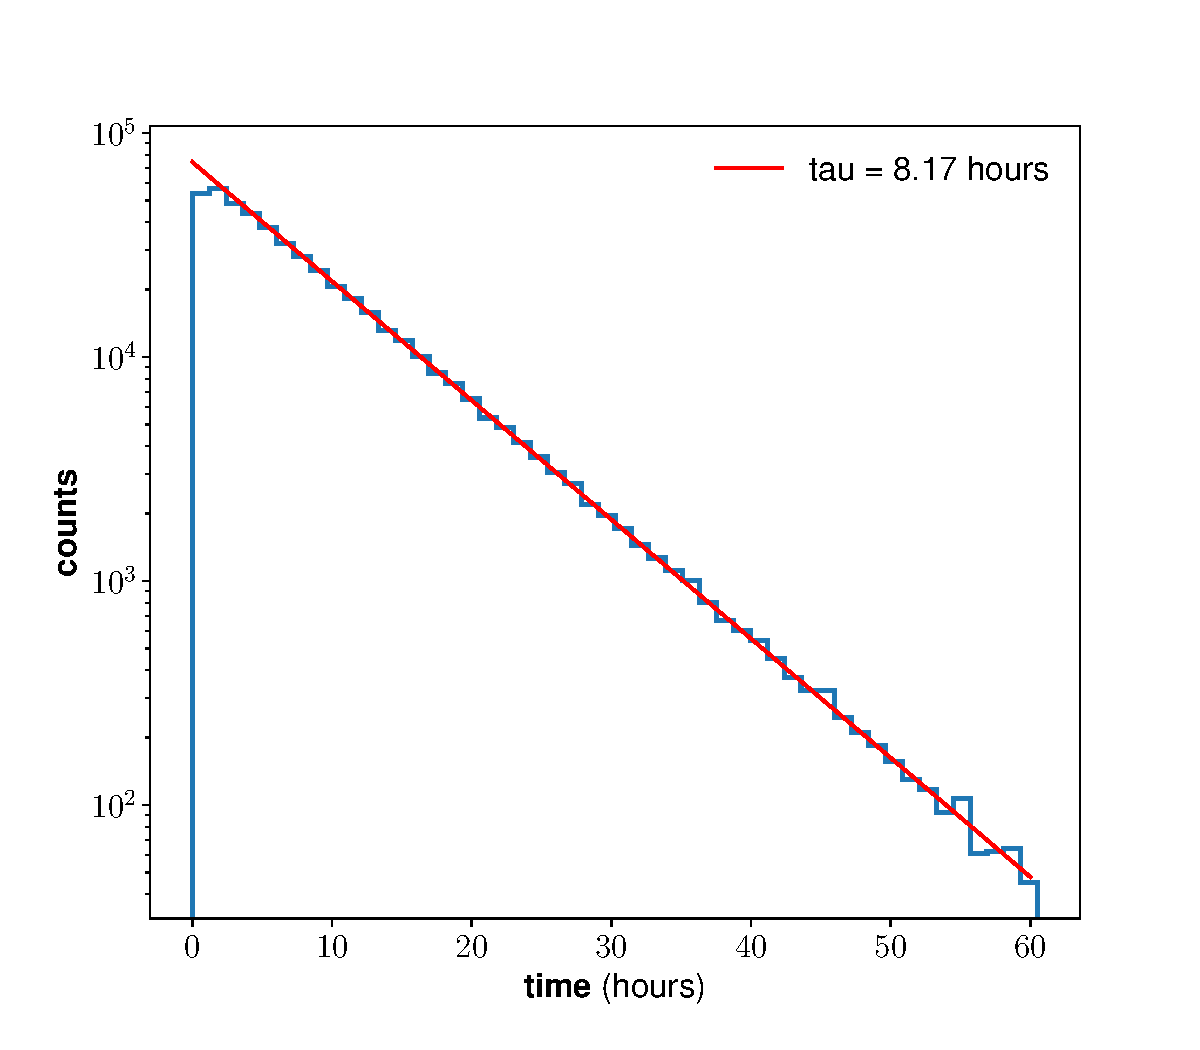
\includegraphics[width=\textwidth]{Figures/H3_removal_time.pdf}
  %\label{}
\end{subfigure}%
\begin{subfigure}{0.5\textwidth}
  \centering
  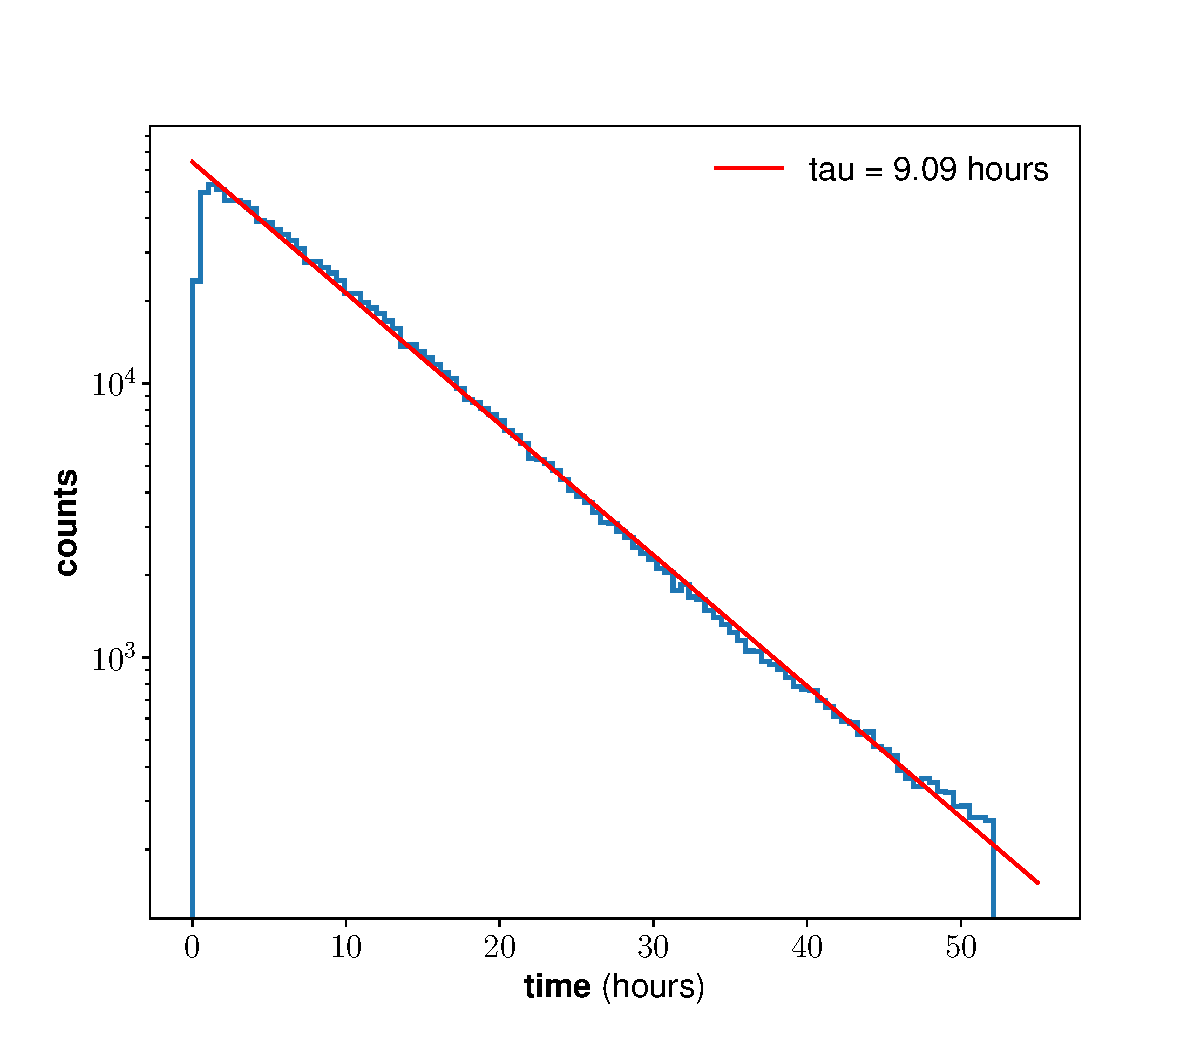
\includegraphics[width=\textwidth]{Figures/C14_removal_time.pdf}
  %\label{fig:intlin}
\end{subfigure}
\caption{Purification of methane radio-labeled with tritium (left), and carbon-14 (right). The tritiated methane is removed with a time constant of 8.2 hours, and the carbon-14 labeled methane is removed with a time constant 9.1 hours. }
\label{fig:removaltime}
\end{figure}




The endpoint of the carbon-14 spectrum is obscured by the xenon-131m line. We don not assume that gammas and betas behave in the same way in liquid xenon, so we need to cut out the xenon-131m events in order to measure the energy deposition properties of carbon-14. At 145 keV, the xenon distribution falls to less than 5\% of the carbon-14 distribution, so we will only include events with reconstructed energy $<145$ keV in our measurement of the carbon-14 yields and recombination..
\begin{figure}[h!]
\centering
  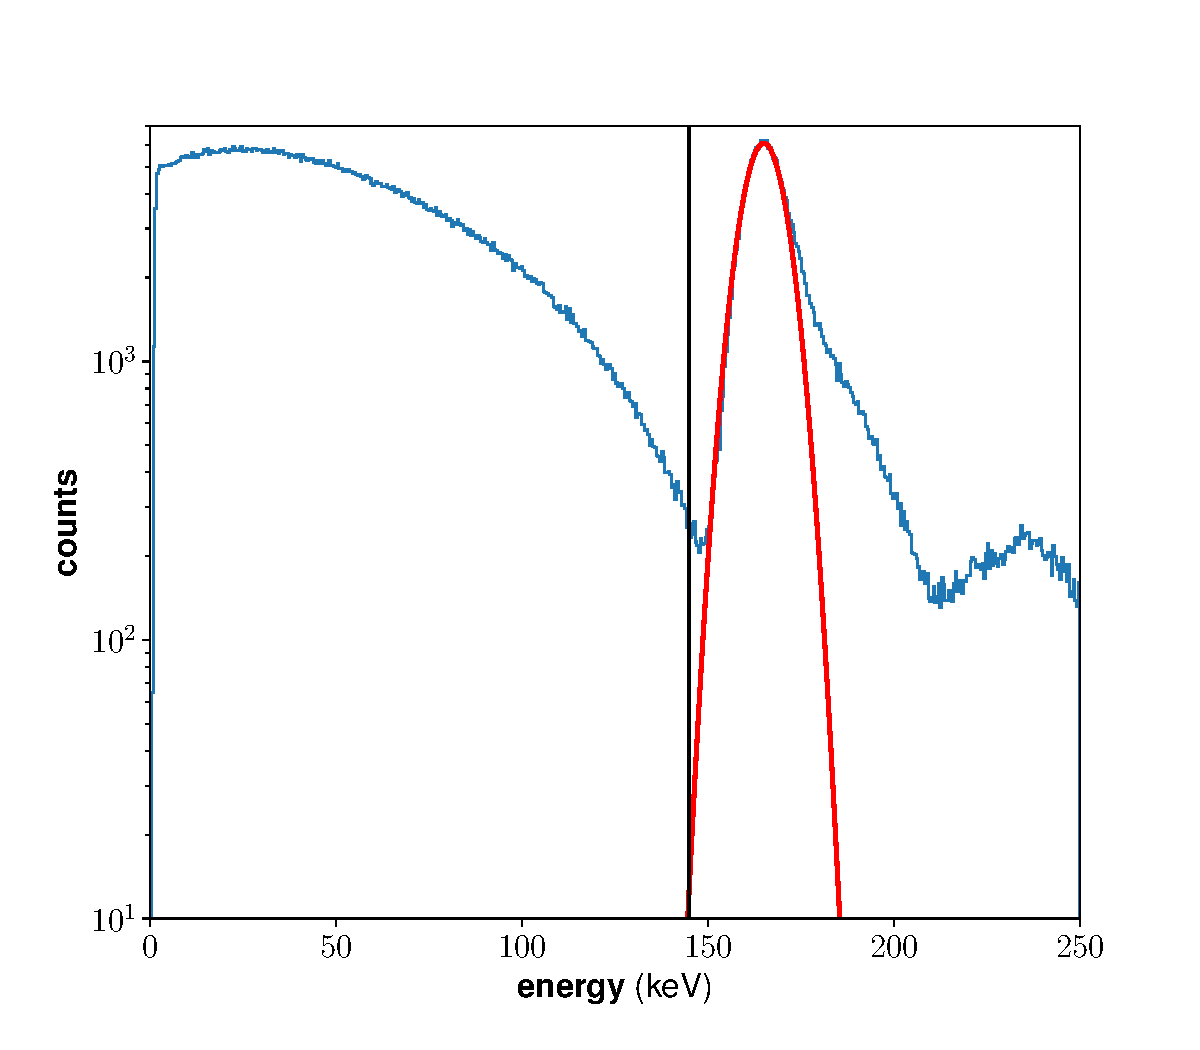
\includegraphics[width=\textwidth]{Figures/C14_spec_init.pdf}
\caption{Reconstructed energy spectrum of the carbon-14 calibration. The blue histogram was generated using all of the events in the dataset, including both carbon-14 and Xe-131m. Most of the events are in the smooth carbon-14 beta spectrum, which extends from 0 to 156 keV, but the Xe-131m line is clearly visible at 164 keV. The red curve shows a Gaussian fit to the xenon-131m spectrum, excluding the high energy side. The black line shows our energy cut at 145 keV.}
\label{fig:c14Ecut}
\end{figure}



\section{The Theoretical $^{14}$C Beta-Spectrum}
The shape of the theoretical spectrum of the carbon-14 beta decay has been of interest in the context neutrino mass experiments\cite{C14_Wietfeldt}, where the goal is to measure the precise endpoint, and in liquid scintillator experiments, which have $^{14}$C as a major background and so need to model the spectrum with high precision\cite{C14_Borexino, C14_Bergeron}. This  decay also is of interest in theoretical nuclear physics because it has an abnormally long half life\cite{C14_Kuzminov,C14_Genz,C14_Garcia}. The transition of $^{14}$C to the ground state of $^{14}$N is an allowed Gamow-Teller $(0^+ \rightarrow 1^+)$ transition. The 5730 year half-life, and corresponding comparative half life, $\log_{10}(f_t)=9.04$, makes it empirically consistent with second-forbidden transitions\cite{C14_Kuzminov,C14_Wietfeldt}.

This extended half life indicates an anomalously small Gamow-Teller nuclear matrix element of $\langle GT \rangle \approx 2 \times 10^{-3}$. This points to cancellation in the lowest order terms of the nuclear matrix element and means that higher order terms must be taken into consideration. These higher-order terms may introduce momentum-dependent deviations from the allowed spectral shape. There have been several experiments\cite{C14_Sonntag, C14_Wietfeldt, C14_Borexino, C14_Kuzminov, C14_Bergeron} which have made measurements of the spectral shape which are consistent with non-statistical corrections to the allowed shape. These results are in some tension with each other, as well as with previous measurements which show a purely allowed spectral shape\cite{C14_Curran}. 

\subsection{The Allowed Spectrum}
Carbon-14 decays to the ground state of nitrogen-14 by way of an allowed Gamow-Teller, 0$^+$ to 1$^+$ transition. This decay has a Q-value of 156 keV and a half life of 5730 years. In general, the theoretical spectrum for this decay takes the form\cite{C14_Kuzminov}:
\begin{equation}\label{eq:beta_spec}
\frac{dN}{dE}=\frac{1}{2\pi^3} \xi C(E) F(Z,E) pE(E_0-E)^2
\end{equation}
Here, $p$ and $E$ are the momentum and total energy of the emitted beta, and $E_0$ is the endpoint energy of the spectrum. In equation \ref{eq:beta_spec} we have neglected the neutrino mass as well as a radiative correction term which is expected to have $<1\%$ effect on the shape of the spectrum\cite{C14_Wietfeldt}. The initial distribution of momentum between the electron and neutrino is proportional to $pE(E_0-E)^2$. This is derived by the phase space density of free particles and will be referred to as the phase space factor. The Fermi function $F(Z,E)$ contains information about the interaction between the emitted beta and the daughter nucleus. The terms $\xi$ and  $C(E)$ represent the energy independent and energy independent parts of the nuclear matrix element.

\subsection{The Fermi Function}\label{sec:fermifunc}
As the emitted beta travels away from the daughter nucleus, the two interact and either increase or decrease the momentum of the beta, depending on its charge. In the case of $^{14}C$, the beta has a negative charge and has to climb up out of the electric potential created by the $^{14}N$ daughter nucleus. The resulting observed beta spectrum will then be pulled to lower energy than the initial phase space factor. This modification to the spectrum if known as the Fermi function, $F(Z,E)$. The traditional derivation of $F(Z,E)$ begins by assuming the daughter nucleus is a fixed point charge and then evaluates the electron wave-function given the resulting field. The wave function is only evaluated down to the nuclear radius, $R$, in order to avoid divergence\cite{wilkinson}:
\begin{equation}\label{eq:fermifunc1}
F(Z,E)=2(\gamma+1)\Gamma(2\gamma+1)^{-2}(2pR)^{2(\gamma-1)}e^{\pi \alpha Z E/p}|\Gamma(\gamma+i\alpha ZE/p)^{2}|^2
\end{equation}

There is also a much simpler closed-form solution in the low-Z, non-relativistic approximation\cite{beta_fermi}:
\begin{equation}\label{eq:fermifunc2}
F_{NR}(Z,E)=\frac{x}{1-exp(-x)},
\end{equation}
where $x=2\pi Ze^{2}/\hbar v$. Here, $Z$ is the atomic number of the daughter nucleus, $e$ is the electron charge, and $v$ is the final velocity of the beta particle. 

Electrons in the higher-momentum part of the spectrum will have velocities exceeding 0.5c, so the non-relativistic approximation may not hold. This being the case, we consider the Bethe-Bacher approximation, which estimates the relativistic correction\cite{beta_fermi,bethe}:
\begin{equation}\label{eq:fermifunc3}
F_{BB}(Z,E)=F_{NR}(Z,E)[W^2(1+4\gamma^2)-1]^S,
\end{equation}
where $W\equiv E/m_ec^2$, $\gamma \equiv \alpha Z$, and $S\equiv (1-\gamma^2)^{1/2}-1)$. The full relativistic Fermi function can be estimated by a series expansion on powers of $(\alpha Z)$\cite{wilkinson,C14_Wietfeldt}. This sum is of limited use to us here because it becomes invalid at low kinetic energy and in fact diverges at zero.

The final correction to the Fermi function we consider is the correction for screening of the Coulomb potential by the orbital electrons. This essentially amounts to a shift in the origin of $F(Z,E)$\cite{C14_Wietfeldt,beta_screening}:
\begin{equation}\label{eq:fermifunc4}
F_{S}(Z,E)=\frac{E'p'}{Ep}F(Z,E'),
\end{equation}
where $E'=E-V_0$ and $p'$ is is the associated momentum. For the $^{14}$C beta decay, $V_0=495$eV\cite{C14_Wietfeldt}.

Figure \ref{fig:C14_spec_corrs} compares the non-relativistic approximation to the various corrections described in this section. We can see that the Wilkinson expansion differs from $F_{NR}(7,E)$ by less than a percent down to a few eV, at which point it diverges. The Bethe-Bacher approximation is similarly very close to $F_{NR}(7,E)$, but it does not display the same pathological behavior at the origin. The correction for electron screening peaks at 1.5\% at a kinetic energy of $T=3.5$keV. Because of the pathology in the Wilkinson expansion, we will take our Fermi function to be the combination of equations \ref{eq:fermifunc3} and \ref{eq:fermifunc4}:
\begin{equation}\label{eq:fermifunc5}
F(Z,E)=\frac{E'p'}{Ep}F_{NR}(Z,E')[(E'/m_ec^2)^2(1+4\gamma^2)-1]^S,
\end{equation}
with $F_{NR}(Z,E)$ as defined in equation \ref{eq:fermifunc2} and $E'$ and $p'$ as defined for eqaution \ref{eq:fermifunc4}.

\begin{figure}[h!]
\centering
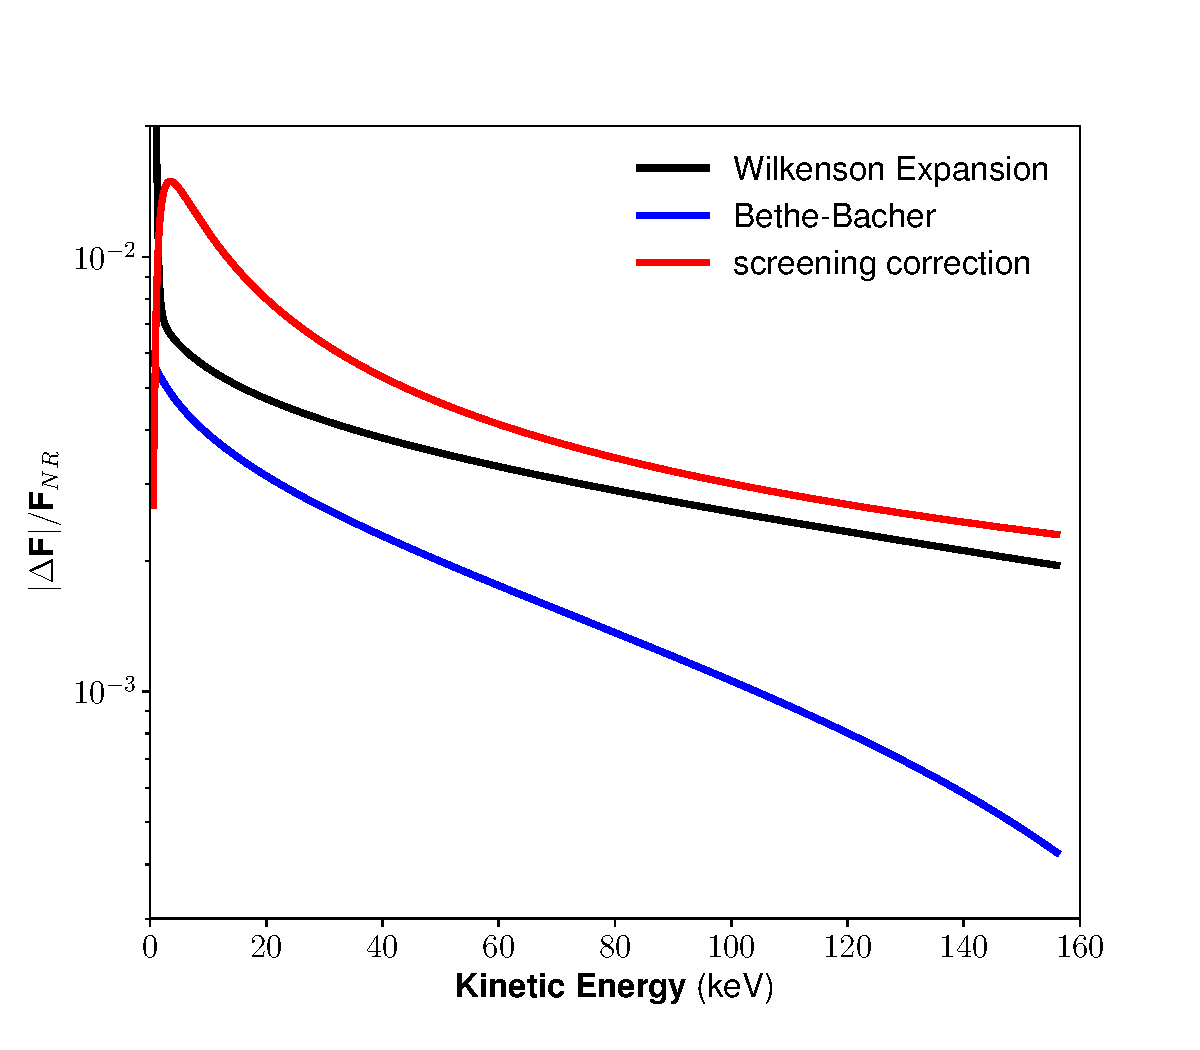
\includegraphics[width=\textwidth]{Figures/FermiFunc_compare.pdf}
\caption{Correction factors for the $^{14}$C beta Fermi function. We compare the non-relativistic approximation, $F_{NR}(7,E)$ to the relativistic corrections described in section \ref{sec:fermifunc}, as well as the non-relativistic function after having been adjusted to account for screening by the orbital electrons. Plotted is $|F'(7,E)-F_{NR}(7,E)|/F_{NR}(7,E)$, where $F'(7,E)$ are the adjusted Fermi functions as indicated in the legend.} 
\label{fig:C14_spec_corrs}
\end{figure}

\subsection{The Shape Factor}\label{sec:shape_factor}
For a typical allowed decay, the shape factor is dominated by interference between the Gammow-Teller axial matrix element, $\langle GT \rangle$ and the weak magnetism matrix element, $\langle WM \rangle$. Such a shape factor has the form\cite{C14_Kuzminov,C14_Garcia,C14_Wietfeldt,beta_Calaprice}:
\begin{equation}\label{eq:shapefactor1}
C(E)\approx1+\frac{4}{3M}\frac{\langle WM \rangle}{\langle GT \rangle}[E-E_0/2-m_e^2/E],
\end{equation}
where $M$ is the nucleon mass, $m_e$ is the electron mass, and $E_0$ is the endpoint energy of the beta-spectrum. Usually the energy dependence of $C(E)$ is small enough that it can be neglected, but in the $^{14}$C beta decay the suppressed decay rate means that $\langle GT \rangle$ is small enough to make its consideration necessary. Under the conserved vector current hypothesis (CVC), the weak magnetism matrix element can be analogized to that of an M1 electromagnetic transition ($\langle WM \rangle$=$\langle M1 \rangle$) for the purpose of calculating the expected shape factor. The ground state of $^{14}$C is an element of an isospin triplet, together with the $^{14}$O ground state and the first excited state of $^{14}$N. The M1 transition is the same as that of the first excited state of $^{14}$N transitioning to the ground state.

There have been several calculations of the predicted shape factor\cite{C14_Garcia,C14_Wietfeldt,C14_Genz}. These typically use a more general form of the $C(E)$ which takes into account terms which have been neglected from equation \ref{eq:shapefactor1}:
\begin{equation}\label{eq:shapefactor2}
C(E)=1+aE+\mu_1\gamma_1b/E+cE^2,
\end{equation}
where $\gamma_1=[1+(\alpha Z)^2]^{1/2}$ and $\mu_1$ is a special Coulomb function. The coefficients $a$, $b$, and $c$ can be calculated using the appropriate matrix elements. The matrix elements are typically calculated using model wave functions for the $^{14}$C and $^{14}$N ground states.

The first measurement of the $^{14}$C shape factor was made by Sonntag et. al. in 1970\cite{C14_Sonntag}. In units of MeV, his measured shape factor was, $C(E)=1-9.14E+1.53/E+7.66E^2$. Genz et. al.\cite{C14_Genz} used this result in part to derive phenomenological wave functions which replicate the shape factor. Later experiments and theoretical calculations have rejected this shape factor.

Wietfeldt et. al. found their data to be consistent with a shape factor of $C(E)=1+aE$, with $a=-0.45 \text{ \ MeV}^{-1}$\cite{C14_Wietfeldt}. This result is very close to their own theoretical calculation of $a=-0.38 \pm 0.04 \text{ \ MeV}^{-1}$, along with theoretical calculations by Garcia and Brown\cite{C14_Garcia}, and  Calaprice and Holstein\cite{beta_Calaprice}. However, the best-fit value of $a$ was inconsistent depending on what range of energies was fit, and a second measurement of the spectrum 2 years later yielded a best fit parameter of $a=-0.63 \pm 0.05 \text{ \ MeV}^{-1}$. 

The Borexino collaboration attempted to measure the shape of the $^{14}$C beta spectrum using their counting test facility (CTF). They assumed the same functional form as the Wietfeldt paper and excluded all $a<-0.72 \text{ \ MeV}^{-1}$ with 90\% confidence\cite{C14_Borexino}. 


Most recently, V. Kuzminov and N. Osetrova measured the shape factor of then $^{14}$C beta decay using a wall-less proportional counter\cite{C14_Kuzminov}. They assumed a shape factor with the form, $C(E)=1+\beta(Q-T)$, with $Q$ being the endpoint energy and $T$ being the kinetic energy of the electron. They measured $\beta=1.24 \pm0.04 \text{ \ MeV}^{-1}$, which is in agreement with a theoretical calculation by Genz et. al.\cite{C14_Genz}. This result is equivalent to $a=-0.68 \pm0.02 \text{ \ MeV}^{-1}$ in a Wietfeldt-style shape factor and is very close to both the Borexino measured limit, as well as the second Wietfeldt measurement.

\begin{figure}[h!]
\centering
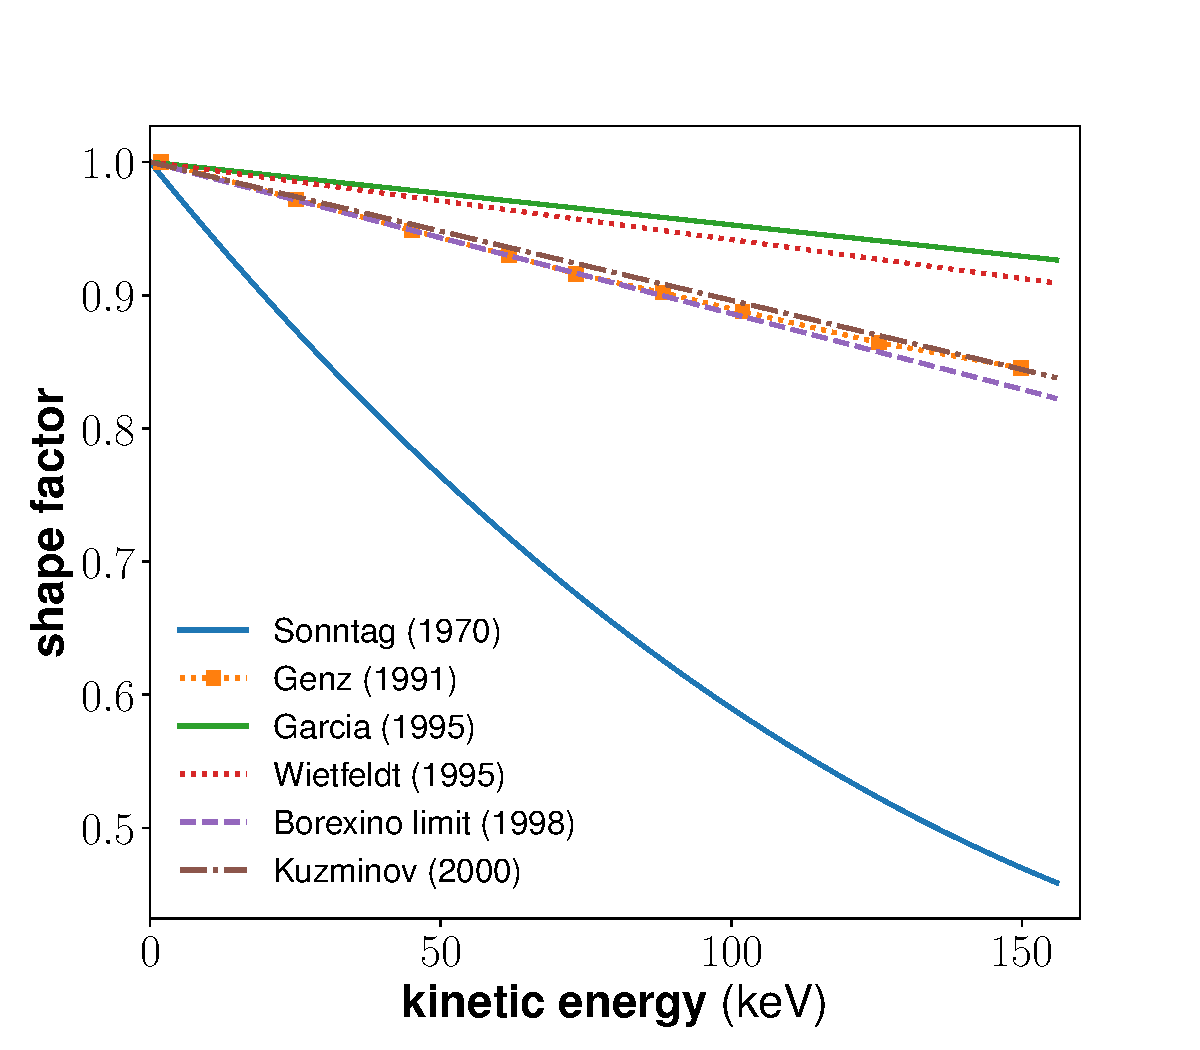
\includegraphics[width=\textwidth]{Figures/ShapeFac_compare.pdf}
\caption{Various measurements and theoretical calculations of the $^{14}$C shape factor. They have all been normalized to equal 1 at kinetic energy=0 keV. The Sonntag\cite{C14_Sonntag}, Wietfeldt\cite{C14_Wietfeldt}, Borexino\cite{C14_Borexino}, and Kuzminov\cite{C14_Kuzminov} lines are all experimental measurements, while the Genz\cite{C14_Genz} and Garcia\cite{C14_Garcia} lines are theoretical calculations. It is clear that the Sonntag result is strongly disfavored by all subsequent experiments and theoretical calculations. This figure also shows Genz, Borexino, Kuzminov, as well as the second Wietfeldt result (not shown) all converging around $C(E)\approx 1-(0.7 \text{ \ MeV}^{-1})E$. It would be difficult, however, to claim this as consensus because the only true measurement in this subset is the Kuzminov line. Neither the Borexino paper nor the Wietfeldt paper claim a strong measurement of the shape factor.} 
\label{fig:C14_shape}
\end{figure}



\section{Preliminary Measurement of Light and Charge Yields}
The carbon-14 injection was based on the tritium calibration, which was first performed in August of 2013, after the first LUX data run was completed. The data from this calibration was used to calculate the energy deposition properties of electronic recoils in liquid xenon. To this end, a method was developed by Attila Dobi which deconvolved the effects of detector-resolution from the interesting physics involved in the process\cite{lux_tritium,attila}. 

Unfortunately this method, which we will refer to as the Dobi method, is largely irrelevant to the post-Run04 data. It relies on a robust understanding of the detector resolution and uses a Gaussian model of the energy smearing to obtain the necessary corrections. The S2 tails described in section \ref{sec:s2tails} were not present in the LUX Run03 data and mean both that our understanding of the energy-dependent detector resolution is limited and that the Gaussian model will not apply. To address these issues, we will develop a numerical version of the Dobi method using our modified version of libNEST which includes the empirical model of the S2 tails. 


\subsection{Accounting for Gaussian Smearing of Continuous Beta Spectra}
This deconvolution of detector resolution is necessary because of the continuous nature of beta spectra. We do not know the true deposition energy, $E_{true}$, of any given event and therefore only have access to the reconstructed energy, $E_{rec}$. In the Run03 measurements, the reconstructed energy of any event would be drawn from a Gaussian distribution centered at the true deposition energy, with the width of this distribution being the energy resolution, $\sigma_{E}$. 
\begin{figure}[h!]
\centering
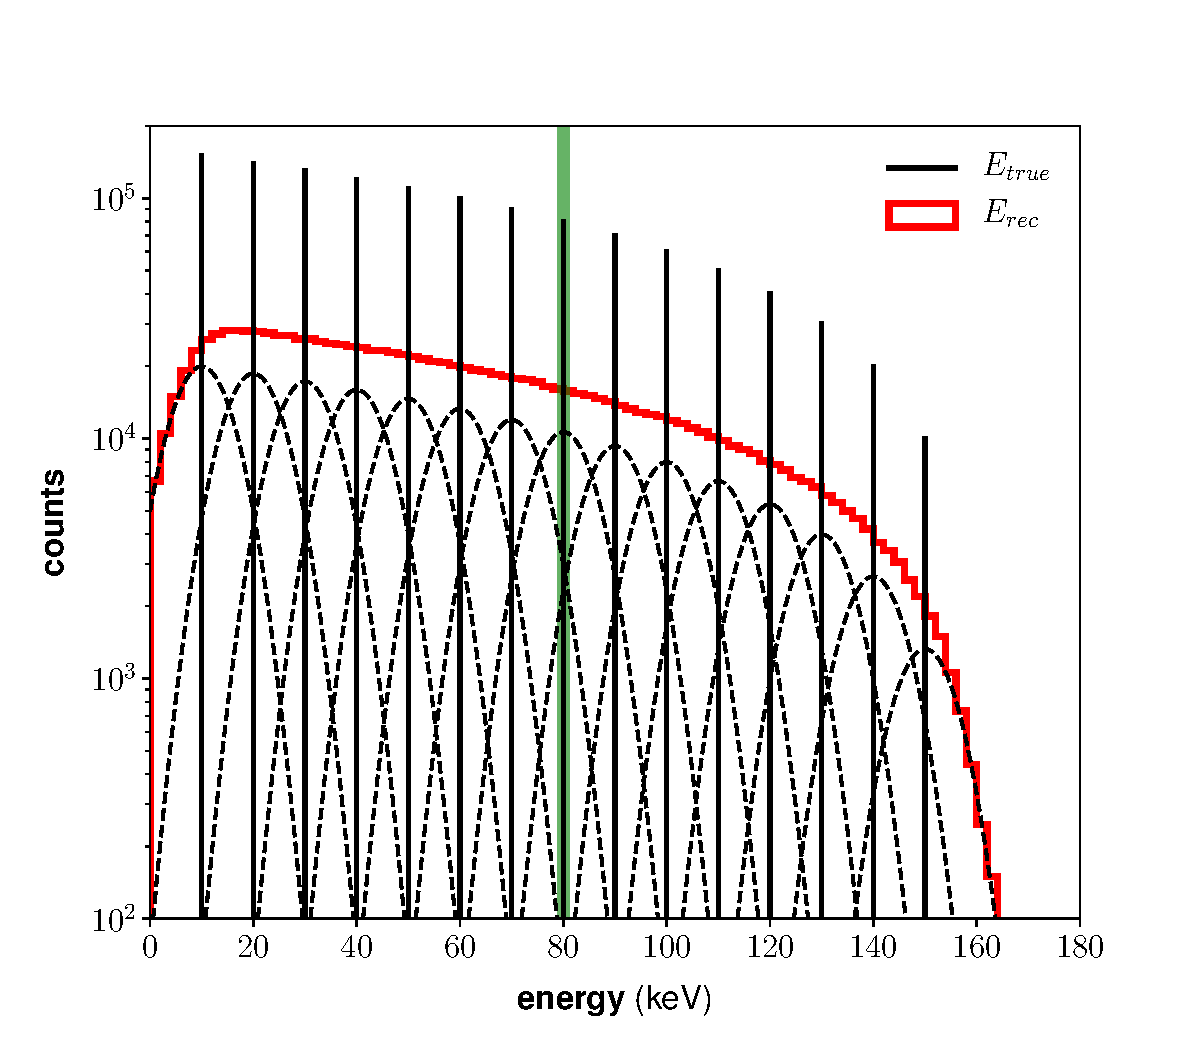
\includegraphics[width=\textwidth]{Figures/toy_smearing.pdf}
\caption{Smearing of a discrete, linearly falling spectrum. The true energy of the events is distributed at ( 10, 20, 30, ... ,150 ) keV, as indicated by the solid black lines. The number of events at each energy decreases linearly. We then apply Gaussian smearing with a flat resolution of 6 keV to the true energy (dashed lines). The reconstructed energy (red histogram) shows the resulting spectrum. The average true energy of events in a slice from 79.75 keV $<E_{rec}<$ 80.25 keV (green area) is 70.65 $\pm$0.09 keV. This average is offset from the selected energy due to smearing.}
\label{fig:toysmear}
\end{figure}

When this Gaussian smearing is applied to a continuous spectrum with a non-zero slope, it will create a systematic offset the measured reconstructed energy from the true energy. We take the spectrum shown in figure \ref{fig:toysmear} as an example. The true energy of the events is distributed at discrete energies, 10, 20, 30, up to 150 keV. We apply Gaussian smearing with a constant resolution of $\sigma_{E}$= 6 keV to give us our reconstructed energy spectrum. When we take a small slice in reconstructed energy, from 79.75 to 80.25 keV, we find that the average true energy of events in this slice is systematically offset to 79.53 $\pm$0.09 keV. This offset is due to the negative slope of the true energy spectrum. The lower energy bins are more prominent than the higher energy ones, and therefore will have more events smear into our reconstructed energy slice.

It is possible to calculate this offset explicitly by integrating the contribution from each individual Gaussian. The number of events contributed to our reconstructed energy slice by the $i^{th}$ true energy bin will be given by:
\begin{equation}\label{eq:smear1}
\begin{split}
A_i&=\int_{79.75}^{80.25}dx\frac{N_i}{\sqrt{2\pi \sigma_{E}^{2}}} e^{-(x-E_{true,i})^2/2\sigma_{E}^{2}}\\
&=\frac{N_i}{2} \Bigg(\text{erf} \bigg(\frac{80.25-E_{true,i}}{\sqrt{2\sigma_E^2}}\bigg)-\text{erf} \bigg(\frac{79.75-E_{true,i}}{\sqrt{2\sigma_E^2}}\bigg)\Bigg)
\end{split}
\end{equation}
where, $N_i=C(16-i)$ is the number of events in the $i^{th}$ bin, and $C$ is a scaling constant. The expected mean true energy, $\nu_{slice}$, of events in the slice will then be given by:
\begin{equation}\label{eq:smear2}
\nu_{80}=\frac{\sum_i E_{true,i}A_i}{\sum_i A_i}
\end{equation}
For the stated values of $N_i$, $E_{true,i}$, and $\sigma_E$, equation \ref{eq:smear} yields $\nu_{80}=79.56$ keV, which is consistent with the result found in the previous paragraph.  

Equation \ref{eq:smear} can be used to recenter an arbitrary reconstructed energy bin. This correction will be most important for energy regions where the spectrum in question is steeply changing and at its endpoints. For instance, if we take a reconstructed energy slice of our toy spectrum from 149.75 to 150.25 keV, the predicted low-energy bias goes from 0.44 keV as it was for the 80 keV slice, to 3.5 keV. This prediction is consistent with the measured bias of 3.4 $\pm$0.2 keV.

We can generalize equations \ref{eq:smear1} and \ref{eq:smear2} to apply to decays with continuous energy spectra. If the energy resolution of the detector, $\sigma_E(E)$, and the shape of the spectrum, $\frac{dN}{dE}$, are both known, equations \ref{eq:smear1} and \ref{eq:smear2} can be rewritten:
\begin{equation}\label{eq:smear3}
A(B_1,B_2)=\frac{1}{2}\frac{dN}{dE} \Bigg(\text{erf} \bigg(\frac{B_2-E}{\sqrt{2\sigma_E(E)^2}}\bigg)-\text{erf}\bigg(\frac{B_1-E}{\sqrt{2\sigma_E(E)^2}}\bigg)\Bigg),
\end{equation}
and:
\begin{equation}\label{eq:smear4}
\nu(B_1,B_2)=\frac{\int A(B_1,B_2)EdE}{\int A(B_1,B_2)dE},
\end{equation}
where $B_1$ and $B_2$ are the edges of the reconstructed energy slice. The calculated $\nu(B_1,B_2)$ can then be used to recenter the arbitrary reconstructed energy bin to the average true energy of events in that bin.

\subsection{Accounting for Non-Gaussian Smearing }
The results from the previous section, shown in equations \ref{eq:smear3} and \ref{eq:smear4} provide a powerful correction method for experiments with Gaussian detector resolution. Unfortunately, the resolution of LUX Run04 and post-Run4 data is not Gaussian. The pathological S2 tails make the resolutions approximately exponential to the high-energy side while leaving it roughly Gaussian on the low-energy side. 

The asymmetry combined with the extended range of the resolution severely limit the effectiveness of equations \ref{eq:smear3} and \ref{eq:smear4}. For this reason, we move from an analytical approach to a numerical one. The libNEST model has been fine-tuned to replicate the LUX detector resolution, so we will combine it with the model of the S2 tails described in section \ref{sec:s2tails} to un-smear the data. 


\section{Measurement of Recombination Fluctuations from $^{14}$C}

\begin{equation}
\sigma_{R}^2=R(1-R)\cdot N_i +\bigg(F_0\exp \Big(\frac{-(Y-F_1)^2}{2F_2^2}\Big)\bigg)^2N_i^2
\end{equation}


\section{Yields and Recombination from Updated NEST Model}


\section{Measurement of the Shape of the $^{14}$C Beta-Spectrum}


















